%%%%%%%%%%%%%%%%%%%%%%%%%%%%%%%%%%%%%%%%%%%%%%%%%%%%%%%%%%%%%%%%%%%%%%
% Overleaf (WriteLaTeX) Example: Molecular Chemistry Presentation
%
% Source: http://www.overleaf.com
%
% In these slides we show how Overleaf can be used with standard 
% chemistry packages to easily create professional presentations.
% 
% Feel free to distribute this example, but please keep the referral
% to overleaf.com
% 
%%%%%%%%%%%%%%%%%%%%%%%%%%%%%%%%%%%%%%%%%%%%%%%%%%%%%%%%%%%%%%%%%%%%%%

\documentclass{beamer}

\mode<presentation>
{
  \usetheme{Madrid}       % or try default, Darmstadt, Warsaw, ...
  \usecolortheme{default} % or try albatross, beaver, crane, ...
  \usefonttheme{default}    % or try default, structurebold, ...
  \setbeamertemplate{navigation symbols}{}
  \setbeamertemplate{caption}[numbered]
} 

\usepackage[english]{babel}
\usepackage[utf8x]{inputenc}
\usepackage{graphicx}
\usepackage{hyperref}
  \hypersetup{colorlinks=true}
  \hypersetup{urlcolor=blue}
  \hypersetup{linkcolor = .}
\usepackage{xcolor}
\usepackage{siunitx}
  \sisetup{separate-uncertainty = true}
\usepackage{physics}
\usepackage[font=small,labelfont=bf]{caption}
\usepackage{subcaption}
\usepackage[en-GB]{datetime2}
\usepackage{overpic}
\usepackage{feynmp}
\DeclareGraphicsRule{*}{mps}{*}{}

\usepackage{scalerel}
\newcommand{\mylbrace}[2]{\vspace{#2pt}\hspace{6pt}\scaleleftright[\dimexpr5pt+#1\dimexpr0.06pt]{\lbrace}{\rule[\dimexpr2pt-#1\dimexpr0.5pt]{-4pt}{#1pt}}{.}}
\newcommand{\myrbrace}[2]{\vspace{#2pt}\scaleleftright[\dimexpr5pt+#1\dimexpr0.06pt]{.}{\rule[\dimexpr2pt-#1\dimexpr0.5pt]{-4pt}{#1pt}}{\rbrace}\hspace{6pt}}

% Here's where the presentation starts, with the info for the title slide
\title[$B^\pm\to(K^+K^-\pi^+\pi^-)_Dh^\pm$]{Analysis update on \texorpdfstring{$\gamma$}{gamma} measurement in \texorpdfstring{$B^\pm\to(K^+K^-\pi^+\pi^-)_Dh^\pm$}{B to K+K-pi+pi-} decays}
\author{Martin Tat}
\institute{Oxford LHCb}
\date{\today}

\titlegraphic{
\includegraphics[height = 3cm, width = 4cm]{lhcb.jpg}\hspace{2cm}~%
              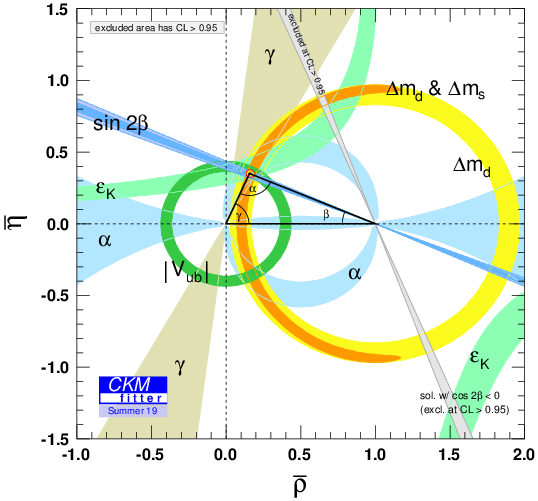
\includegraphics[height = 3cm, width = 4cm]{ckmfitter.png}}

\begin{document}

\begin{frame}
  \titlepage
\end{frame}

% These three lines create an automatically generated table of contents.
\begin{frame}{Outline}
  \tableofcontents
\end{frame}

\section{Introduction (skip)}
\begin{frame}{Introduction (skip)}
  \begin{figure}[H]
    \centering
    \vspace{0.3cm}
    \begin{subfigure}{0.5\textwidth}
      \centering
      \begin{fmffile}{fgraph/fgraph_BtoDK1}
        \setlength{\unitlength}{0.4cm}
        \begin{fmfgraph*}(6,6)
          \fmfstraight
          \fmfleft{i1,B,i2,t1,t2,t3,t9,t10}
          \fmfright{o1,D,o2,t4,t5,o3,K,o4}
          \fmflabel{$\bar{u}$}{i1}
          \fmflabel{$b$}{i2}
          \fmfv{l.d=20,l.a=180,l={$B^-$\mylbrace{30}{-8}}}{B}
          \fmflabel{$\bar{u}$}{o1}
          \fmflabel{$c$}{o2}
          \fmflabel{$\bar{u}$}{o3}
          \fmflabel{$s$}{o4}
          \fmfv{l.d=15,l.a=0,l={\myrbrace{30}{-12}}$D^0$}{D}
          \fmfv{l.d=15,l.a=0,l={\myrbrace{30}{11}}$K^-$}{K}
          \fmf{fermion}{o1,i1}
          \fmf{fermion,tension=1.5}{i2,v1}
          \fmf{fermion}{v1,o2}
          \fmf{phantom,tension=1.5}{t9,v2}
          \fmf{boson,label=$W$,label.side=left,tension=0}{v1,v2}
          \fmf{fermion}{v2,o4}
          \fmf{fermion}{o3,v2}
        \end{fmfgraph*}
      \end{fmffile}
      \vspace{0.5cm}
      \caption{$B^-\to D^0K^-$}
    \end{subfigure}%
    \begin{subfigure}{0.5\textwidth}
      \centering
      \begin{fmffile}{fgraph/fgraph_BtoDK2}
        \setlength{\unitlength}{0.4cm}
        \begin{fmfgraph*}(6,6)
          \fmfstraight
          \fmfleft{i1,t1,t2,B,t9,t10,i2}
          \fmfright{o1,K,o2,t4,t5,o3,D,o4}
          \fmflabel{$\bar{u}$}{i1}
          \fmflabel{$b$}{i2}
          \fmfv{l.d=20,l.a=180,l={$B^-$\mylbrace{100}{-8}}}{B}
          \fmflabel{$\bar{u}$}{o1}
          \fmflabel{$s$}{o2}
          \fmflabel{$\bar{c}$}{o3}
          \fmflabel{$u$}{o4}
          \fmfv{l.d=15,l.a=0,l={\myrbrace{30}{13}}$\bar{D^0}$}{D}
          \fmfv{l.d=15,l.a=0,l={\myrbrace{30}{-13}}$K^-$}{K}
          \fmf{fermion}{o1,i1}
          \fmf{fermion,tension=1.5}{i2,v1}
          \fmf{fermion}{v1,o4}
          \fmf{phantom,tension=1.5}{t2,v2}
          \fmf{boson,label=$W$,label.side=left,tension=0}{v1,v2}
          \fmf{fermion}{v2,o2}
          \fmf{fermion}{o3,v2}
        \end{fmfgraph*}
      \end{fmffile}
      \vspace{0.5cm}
      \caption{$B^-\to\bar{D^0}K^-$}
    \end{subfigure}
  \end{figure}
  \begin{center}
    $\gamma\equiv\text{arg}\Big(-\frac{V_{ud}V^*_{ub}}{V_{cd}V^*_{cb}}\Big)$ \\
    \vspace{0.3cm}
    $b\to u\bar{c}s$ and $b\to u\bar{u}s$ interference when $D^0$ and $\bar{D^0}$ decay into a common final state\\
    \vspace{0.3cm}
    In this analysis, consider $D\to K^+K^-\pi^+\pi^-$
  \end{center}
\end{frame}

\begin{frame}{Introduction (skip)}
  \begin{itemize}
    \item{CP observables:}
    \begin{itemize}
      \item{$x_\pm^{DK} = r_B^{DK}\cos(\delta_B^{DK}\pm\gamma)$}
      \item{$y_\pm^{DK} = r_B^{DK}\sin(\delta_B^{DK}\pm\gamma)$}
      \item{$x_\xi^{D\pi} = \Re(\xi^{D\pi})$, $y_\xi^{D\pi} = \Im(\xi^{D\pi})$ $\quad\quad\Big(\xi^{D\pi} = \frac{r_B^{D\pi}}{r_B^{DK}}e^{i(\delta_B^{D\pi} - \delta_B^{DK})}\Big)$}
    \end{itemize}
  \end{itemize}
  \begin{block}{Event yield in bin $i$}
    $N^-_i = h_{B^-}\Big(K_i + \big(x_-^2 + y_-^2\big)\bar{K_i} + 2\sqrt{K_i\bar{K_i}}\big(x_-c_i + y_-s_i\big)\Big)$
    $N^+_{-i} = h_{B^+}\Big(K_i + \big(x_+^2 + y_+^2\big)\bar{K_i} + 2\sqrt{K_i\bar{K_i}}\big(x_+c_i + y_+s_i\big)\Big)$
  \end{block}
  \begin{block}{Amplitude averaged strong phases and fractional yield}
    $c_i = \frac{\int_i\dd{\Phi}|\mathcal{A}(D^0)||\mathcal{A}(\bar{D^0})|\cos(\delta_D)}{\sqrt{\int_i\dd{\Phi}\abs{\mathcal{A}(D^0)}^2\int_i\dd{\Phi}\abs{\mathcal{A}(\bar{D^0})}^2}}, \quad K_i = \frac{\int_i\dd{\Phi}|\mathcal{A}(D^0)|^2}{\sum_j\int_j\dd{\Phi}\abs{\mathcal{A}(D^0)}^2}$
  \end{block}
\end{frame}

\section{Binning scheme}
\begin{frame}{Binning scheme}
  \begin{itemize}
    \setlength\itemsep{1.2em}
    \item{Use LHCb model (\href{https://arxiv.org/abs/1811.08304}{arXiv:1811.08304}) implemented in AmpGen}
    \item{Calculate $D^0$ and $\bar{D^0}$ amplitude from $D$ daughter momenta}
    \item{$\mathcal{A}(D^0)/\mathcal{A}(\bar{D^0}) = r_D\exp(i\delta_D)$}
    \item{Bin along $\delta_D$ to avoid dilution during averaging}
    \item{Enhance interference by separating bin $+i$ and $-i$ at $r_D = 1$}
    \item{Analogy from $K_S\pi^+\pi^-$: $m^2_+ = m^2_-$ separates CF and DCS resonances}
    \item{Maximize $Q = \frac{1}{2}(Q_+ + Q_-)$ by moving bin boundaries symmetrically around $\delta_D = 0$:}
  \end{itemize}
  \begin{equation*}
    Q_\pm^2 = 1 - \sum_i\frac{K_i\bar{K_i}(1 - c_i^2 - s_i^2)}{N^\pm_i}\Big/\sum_iK_i
  \end{equation*}
\end{frame}

\begin{frame}{Binning scheme}
  \begin{figure}
    \centering
    \vspace{-0.2cm}
    \begin{subfigure}{0.5\textwidth}
      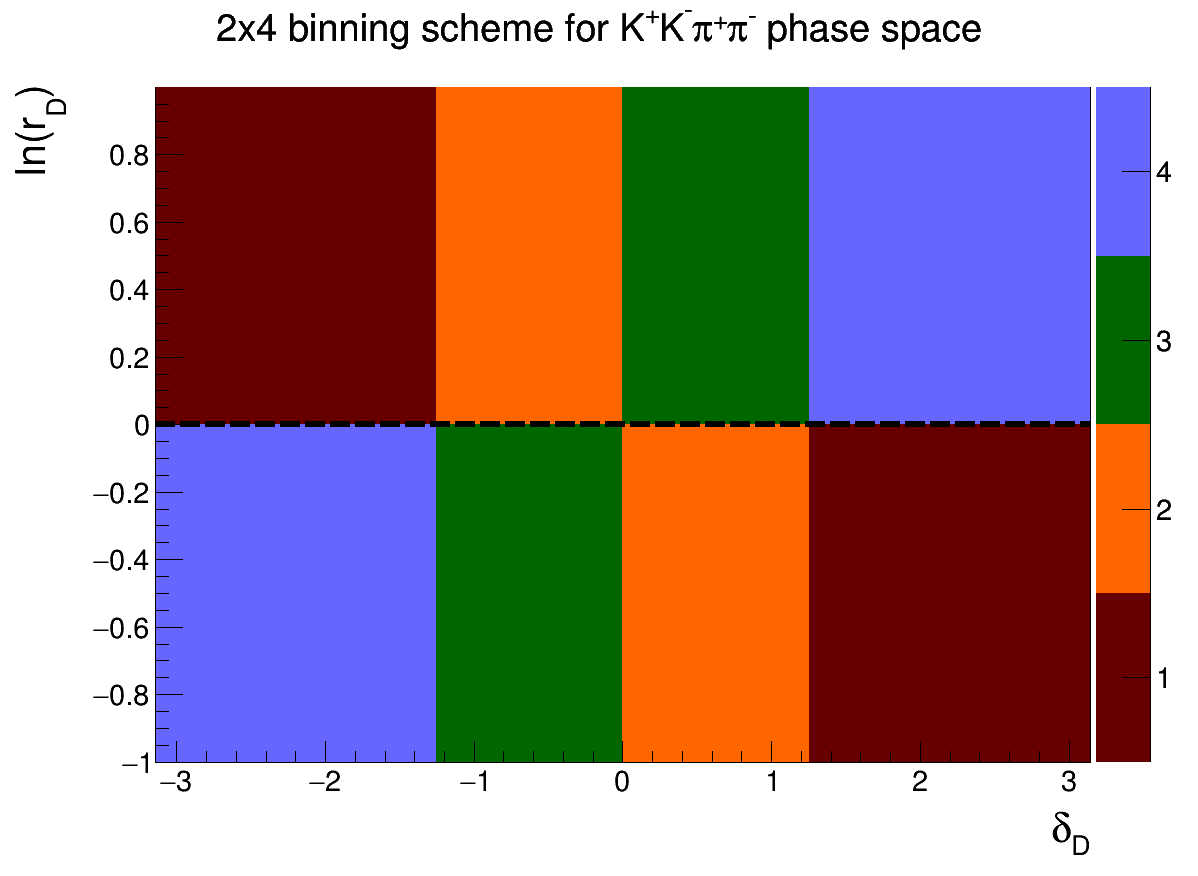
\includegraphics[width = 1.0\textwidth]{Plots/BinningScheme4BinsPlot.png}
      \caption{$2\times 4$ binning scheme \\ $Q = 0.85$}
    \end{subfigure}%
    \begin{subfigure}{0.5\textwidth}
      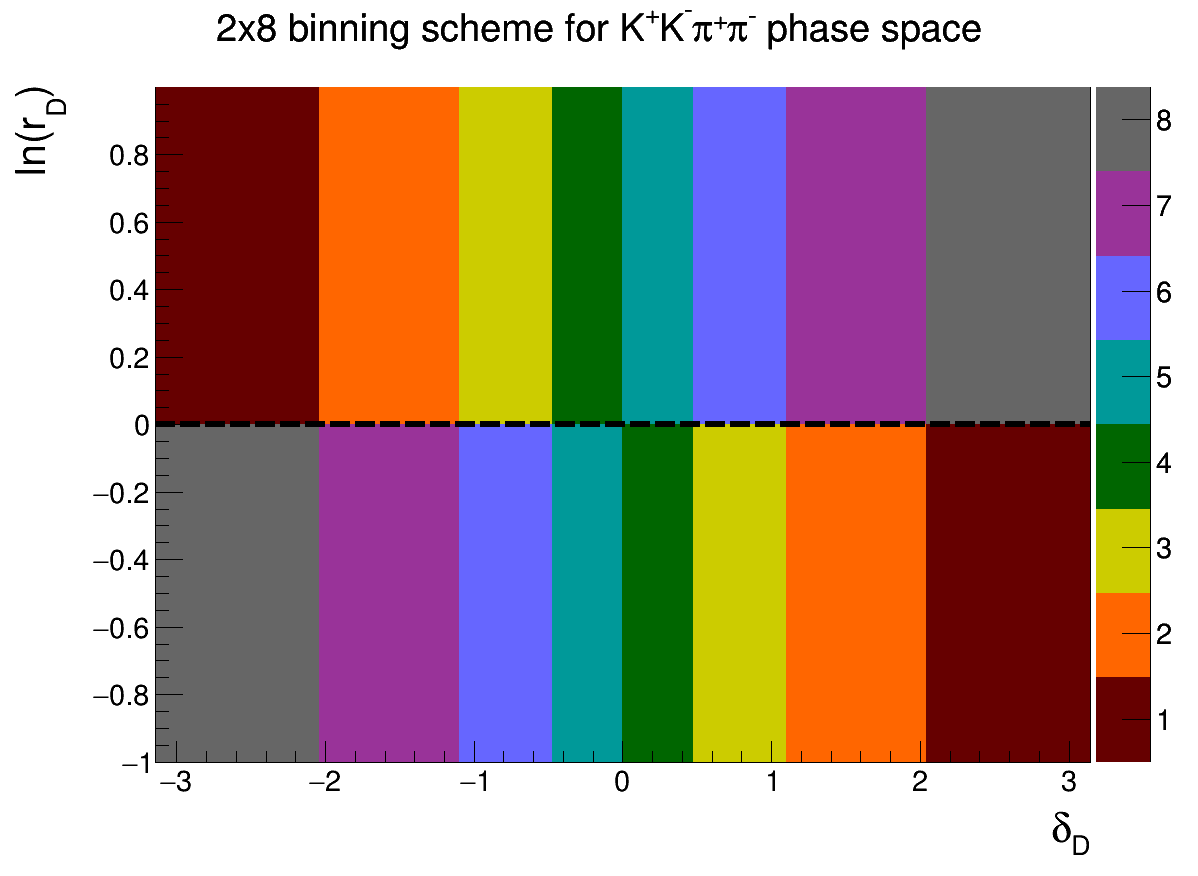
\includegraphics[width = 1.0\textwidth]{Plots/BinningScheme8BinsPlot.png}
      \caption{$2\times 8$ binning scheme \\ $Q = 0.90$}
    \end{subfigure}
  \end{figure}
\end{frame}

\begin{frame}{Strong phases}
  \begin{figure}
    \centering
    \vspace{-0.2cm}
    \begin{subfigure}{0.5\textwidth}
      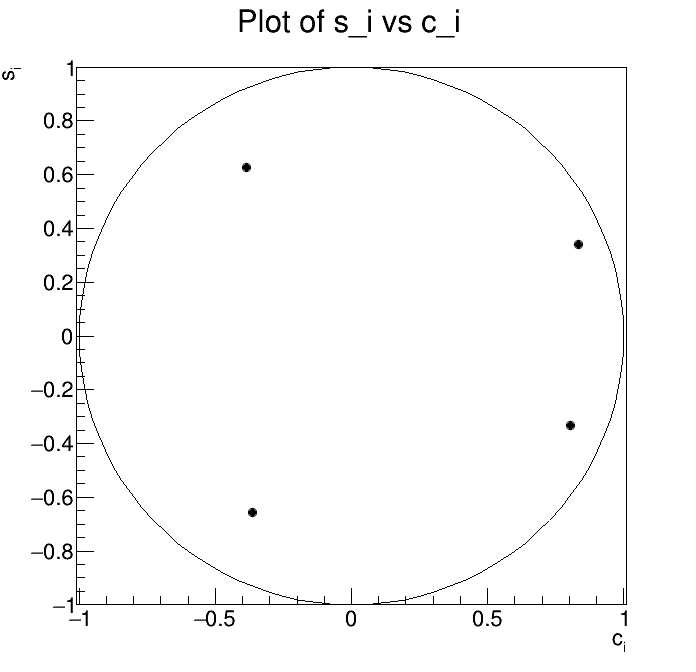
\includegraphics[width = 1.0\textwidth]{Plots/Amplitude_4bins_VariableBins_1p20923_50M_sample1_cs.png}
      \caption{$c_i$ and $s_i$ for the \\$2\times 4$ binning scheme}
    \end{subfigure}%
    \begin{subfigure}{0.5\textwidth}
      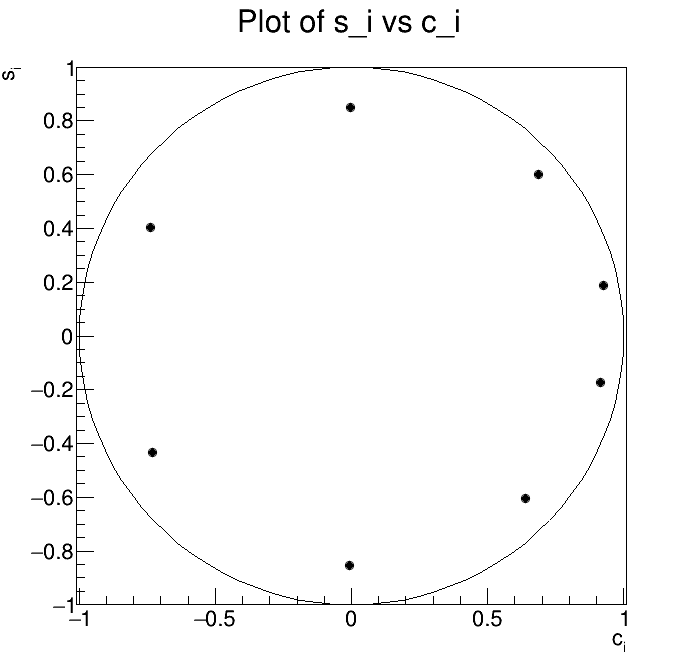
\includegraphics[width = 1.0\textwidth]{Plots/Amplitude_8bins_VariableBins_0p645101_1p72065_2p09644_50M_sample1_cs.png}
      \caption{$c_i$ and $s_i$ for the \\$2\times 8$ binning scheme}
    \end{subfigure}
  \end{figure}
\end{frame}

\begin{frame}{Fractional yields}
  \begin{figure}
    \centering
    \vspace{-0.2cm}
    \begin{subfigure}{0.5\textwidth}
      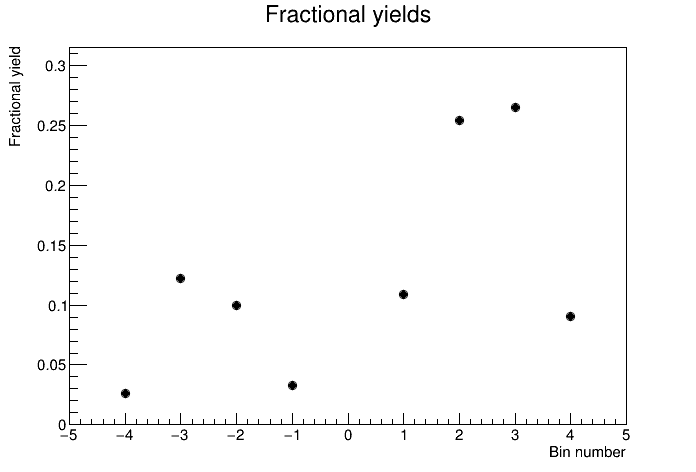
\includegraphics[width = 1.0\textwidth]{Plots/Amplitude_4bins_VariableBins_1p20923_50M_sample1_KKbar.png}
      \caption{$K_i$ for the \\$2\times 4$ binning scheme}
    \end{subfigure}%
    \begin{subfigure}{0.5\textwidth}
      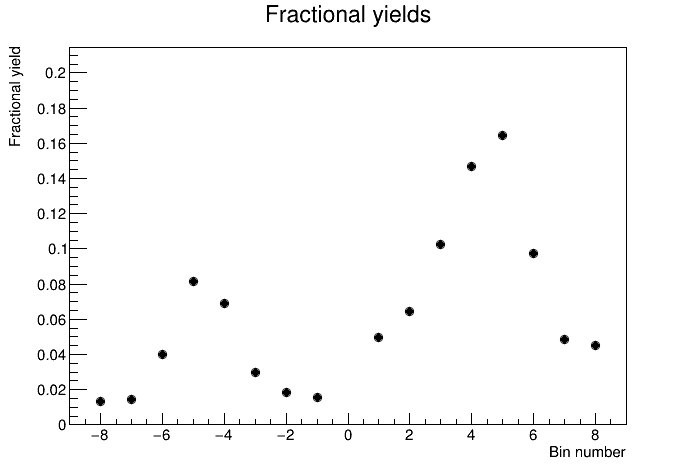
\includegraphics[width = 1.0\textwidth]{Plots/Amplitude_8bins_VariableBins_0p645101_1p72065_2p09644_50M_sample1_KKbar.png}
      \caption{$K_i$ for the \\$2\times 8$ binning scheme}
    \end{subfigure}
  \end{figure}
\end{frame}

\begin{frame}{Study of $\gamma$ precision}
  \begin{itemize}
    \item{Generate $2000$ $B^\pm$ candidates in Ampgen}
    \item{Unbinned fit benchmark: $\Delta\gamma = \SI{11}{\degree}$}
    \item{Both $2\times 4$ and $2\times 8$ binning schemes are consistent with their $Q$ values}
  \end{itemize}
  \begin{figure}
    \centering
    \vspace{-0.2cm}
    \begin{subfigure}{0.5\textwidth}
      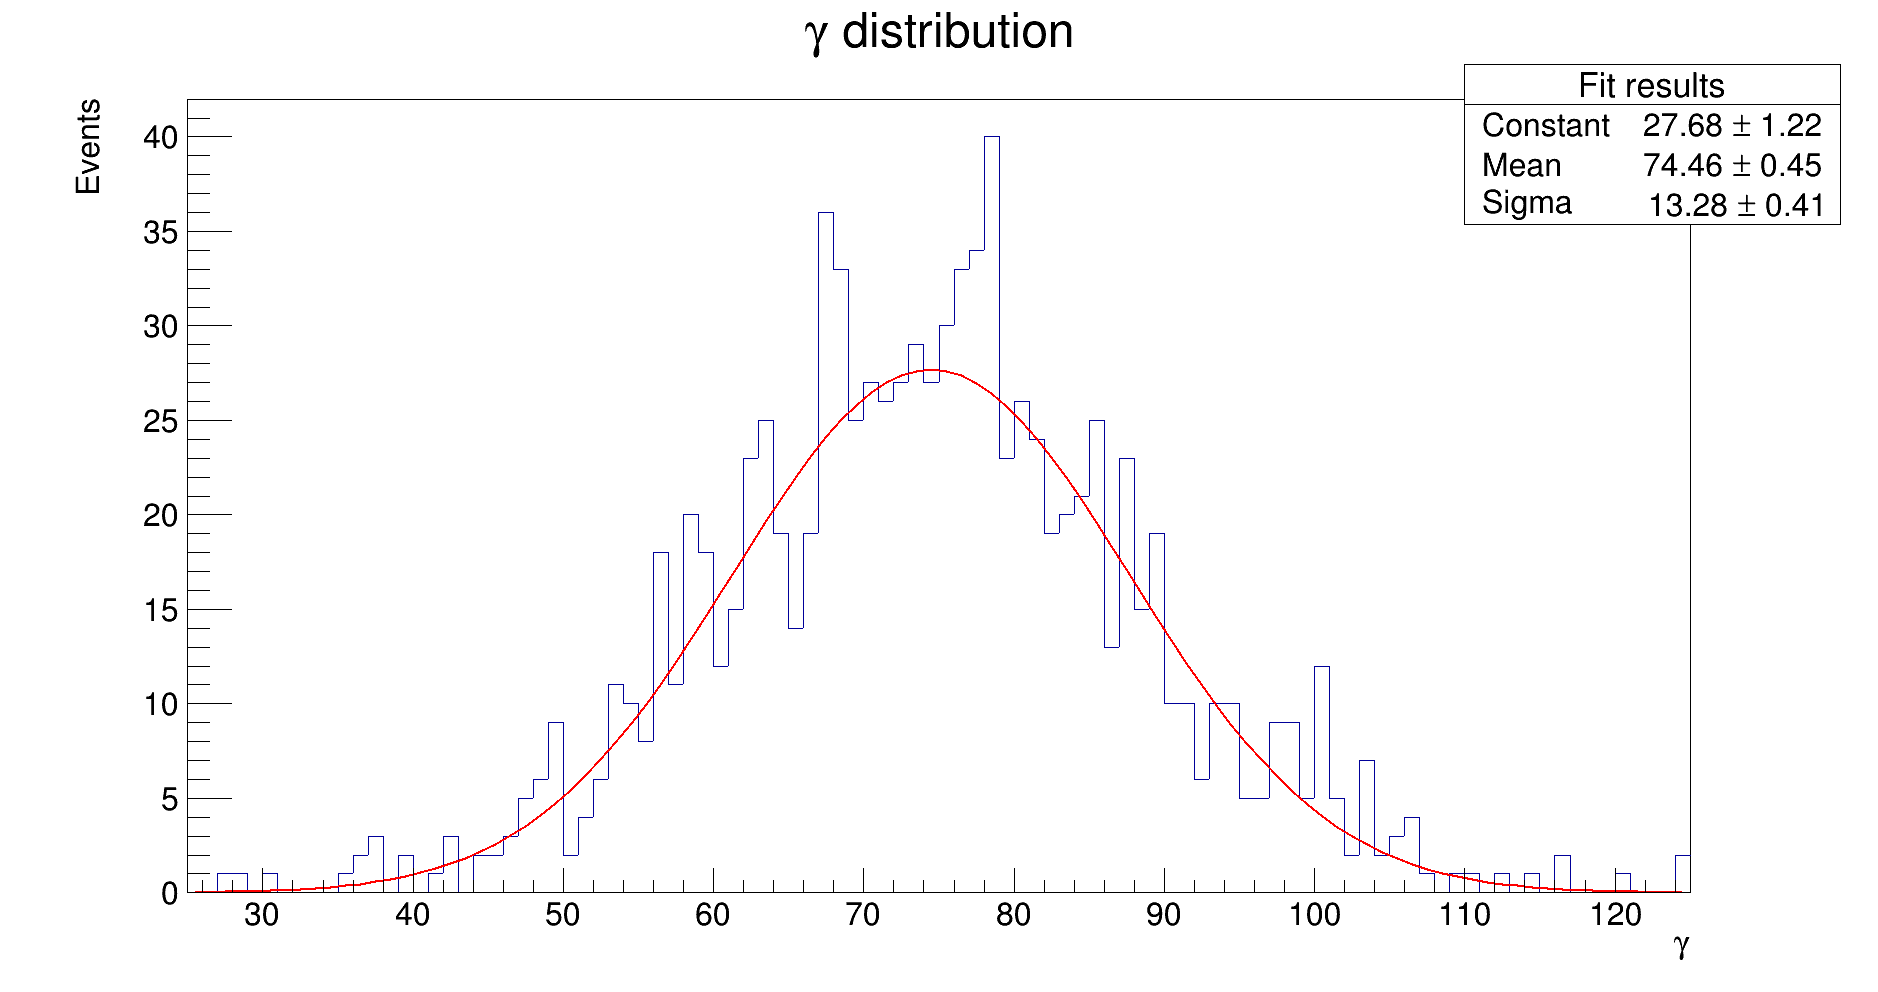
\includegraphics[width = 1.0\textwidth]{Plots/GammaDistribution4BinsVariableWidth.png}
      \caption{$2\times 4$ binning scheme \\ $\Delta\gamma = \SI{13}{\degree}$}
    \end{subfigure}%
    \begin{subfigure}{0.5\textwidth}
      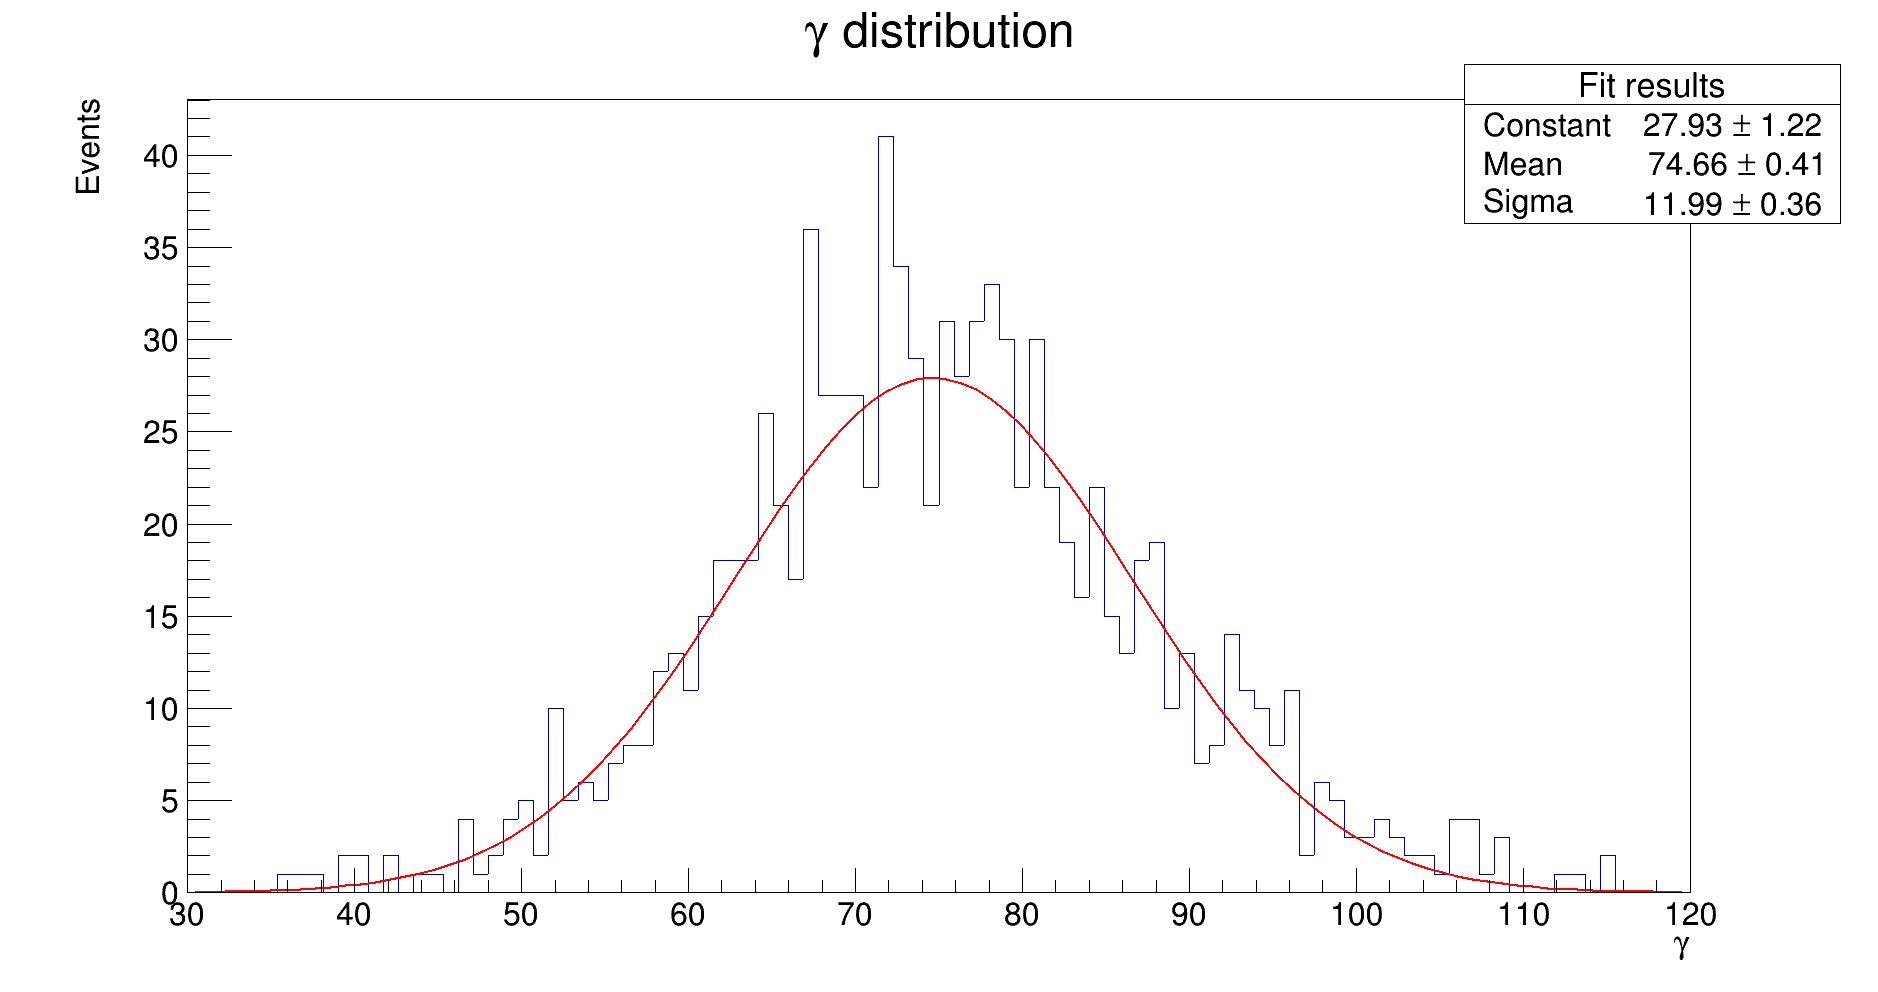
\includegraphics[width = 1.0\textwidth]{Plots/GammaDistribution8BinsVariableWidth.png}
      \caption{$2\times 8$ binning scheme \\ $\Delta\gamma = \SI{12}{\degree}$}
    \end{subfigure}
  \end{figure}
\end{frame}

\section{Summary}
\begin{frame}{Summary}
  Summary:
  \begin{itemize}
    \item{Global and CP fits are working}
    \item{Toy studies show no suspicious behaviour}
  \end{itemize}
  Next steps:
  \begin{itemize}
    \item{Fine tuning the PDF shape parameters and efficiencies?}
  \end{itemize}
\end{frame}

\begin{frame}{Backup slides: DaVinci error}
  \begin{center}
    DaVinci error message:
  \end{center}
  \begin{figure}
    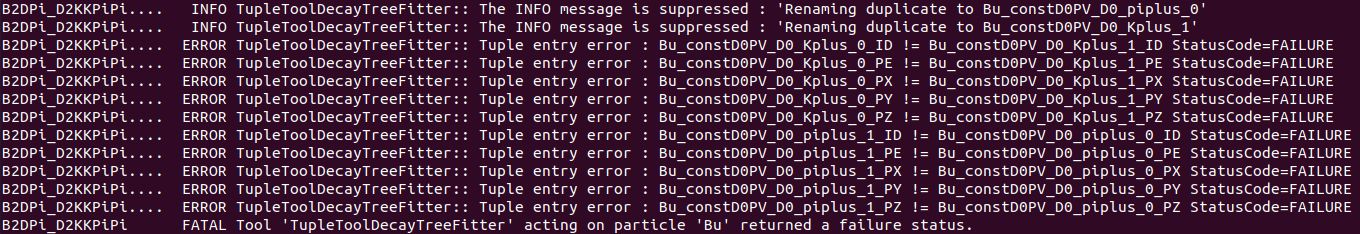
\includegraphics[width = 1\textwidth]{DaVinciError.png}
  \end{figure}
\end{frame}

\end{document}
